\documentclass[11pt]{article}

% ------
% LAYOUT
% ------
\textwidth 165mm %
\textheight 230mm %
\oddsidemargin 0mm %
\evensidemargin 0mm %
\topmargin -15mm %
\parindent= 10mm

\usepackage[dvips]{graphicx}
\usepackage{multirow,multicol}
\usepackage[table]{xcolor}

\usepackage{amssymb}
\usepackage{amsfonts}
\usepackage{amsthm}
\usepackage{amsmath}

\usepackage{subfigure}
\usepackage{minted}

\graphicspath{{./pix/}} % put all your figures here.

\begin{document}
\begin{center}
\Large{\textbf{ECE 595: Homework 4}}

Yi Qiao, Class ID 187

(Spring 2019)
\end{center}

\section*{Exercise 1: Theory}
\subsection*{(a) Logistic regression}
\subsubsection*{(i)}
$$\underset{\pmb{\theta}}{argmin} \sum_{j=1}^{N}-\left\{y_j\log h_{\pmb{\theta}}(\pmb{x}_j)+\left(1-y_j\right) \log (1-h_{\pmb{\theta}}(\pmb{x}_j)) \right\}$$

\begin{equation}
\begin{split}
&=\underset{\pmb{\theta}}{argmin} \sum_{j=1}^{N}-\left\{\log (1-h_{\pmb{\theta}}(\pmb{x}_j))+y_j \log \frac{h_{\pmb{\theta}}(\pmb{x}_j)}{1-h_{\pmb{\theta}}(\pmb{x}_j)} \right\}\\
&=\underset{\pmb{\theta}}{argmin} \sum_{j=1}^{N}-\left\{\log (1-h_{\pmb{\theta}}(\pmb{x}_j))+y_j \log \frac{\frac{1}{1+e^{-\pmb{\theta}^T\pmb{x}_j}}}{\frac{e^{-\pmb{\theta}^T\pmb{x}_j}}{1+e^{-\pmb{\theta}^T\pmb{x}_j}}} \right\}\\
&=\underset{\pmb{\theta}}{argmin} \sum_{j=1}^{N}-\left\{\log(1-h_{\pmb{\theta}}(\pmb{x}_j))+y_j\pmb{\theta}^T\pmb{x}_j \right\}
\end{split}
\end{equation}
Take the derivative..
\begin{equation}
\begin{split}
\nabla_{\pmb{\theta}}\sum_{j=1}^{N}-\left\{\log(1-h_{\pmb{\theta}}(\pmb{x}_j))+y_j\pmb{\theta}^T\pmb{x}_j \right\}&=0\\
\sum_{j=1}^{N}-\left\{\nabla_{\pmb{\theta}}\log(1-h_{\pmb{\theta}}(\pmb{x}_j))+\nabla_{\pmb{\theta}}y_j\pmb{\theta}^T\pmb{x}_j \right\}&=0\\
\sum_{j=1}^{N}\left\{\pmb{x}_jh_{\pmb{\theta}}(\pmb{x}_j)-y_j\pmb{x}_j \right\}&=0\\
\sum_{j=1}^{N}\left\{\left(h_{\pmb{\theta}}(\pmb{x}_j)-y_j\right)\pmb{x}_j \right\}&=0\\
h_{\pmb{\theta}}(\pmb{x}_j)&=y_j
\end{split}
\end{equation}
Which implies, when linearly separable...\\
When $y_j = 1$,
$$\pmb{\theta}^T\pmb{x}_j = \infty$$
When $y_j = 0$,
$$\pmb{\theta}^T\pmb{x}_j = -\infty$$
Since $x_j$ is always bounded, obviously, $\pmb{\theta}$ tends to $\infty$. 
\pagebreak

\noindent Since $\pmb{\theta}$ goes to $\infty$ for $\nabla_{\pmb{\theta}}$ goes to $0$, for any finite $\pmb{\theta}$, the derivative 
$$ \sum_{j=1}^{N}\left\{\left(h_{\pmb{\theta}}(\pmb{x}_j)-y_j\right)\pmb{x}_j \right\}$$
will never goes to $0$. Thus the gradient decent,
$$\pmb{\theta}^{(k+1)}=\pmb{\theta}^{(k)}-\alpha_k\left(\sum_{j=1}^{N}\left(h_{\pmb{\theta}^{(k)}}(\pmb{x}_j)-y_j\right)\pmb{x}_j\right)$$
will never stop for any finite $k$.

\subsubsection*{(ii)}
If linearly separable, the discriminant function will go as steep as possible. Thus, $\pmb{w},\ w_0$ will go as far as possible.\\
We can also add some regularization to the original optimization problem, like
$$\underset{\pmb{\theta}}{argmin} \sum_{j=1}^{N}-\left\{y_j\log h_{\pmb{\theta}}(\pmb{x}_j)+\left(1-y_j\right) \log (1-h_{\pmb{\theta}}(\pmb{x}_j)) \right\}+\lambda||\pmb{\theta}||^2$$

\subsubsection*{(iii)}
No. Since no one else use $\log$ in the loss function.

\subsection*{(b) Perceptron}

\subsubsection*{(i)}

$$\pmb{w}^{(k+1)}=\pmb{w}^{(k)}+y_j\pmb{x}_j,\ some\ j\in \mathcal{M}_k$$

\begin{equation}
\begin{split}
y_j(\pmb{w}^{(k+1)})^T\pmb{x}_j &= y_j(\pmb{w}^{(k)}+y_j\pmb{x}_j)^T\pmb{x}_j\\
&= y_j(\pmb{w}^{(k)})^T\pmb{x}_j+y_j^2\pmb{x}_j^T\pmb{x}_j\\
&= y_j(\pmb{w}^{(k)})^T\pmb{x}_j+y_j^2||\pmb{x}_j||^2_2
\end{split}
\end{equation}

The second term $y_j^2||\pmb{x}_j||^2_2 \ge0$, thus,
$$y_j(\pmb{w}^{(k+1)})^T\pmb{x}_j>y_j(\pmb{w}^{(k)})^T\pmb{x}_j$$

Thus making the loss function smaller.
\pagebreak
\subsubsection*{(ii)} 
\noindent \textbf{Step 1.} Show that $(\pmb{w}^{(k)})^T\pmb{w}^*\ge k\rho$\\
Assuming $\pmb{w}^{(0)} = 0$, obviously, $(\pmb{w}^{(0)})^T\pmb{w}^* = 0 \ge 0\rho$\\
Assuming $(\pmb{w}^{(k-1)})^T\pmb{w}^*\ge (k-1)\rho$,
\begin{equation}
\begin{split}
(\pmb{w}^{(k)})^T\pmb{w}^* &= (\pmb{w}^{(k-1)} + y_j\pmb{x}_j)^T\pmb{w}^*,\ some\ j\in  \mathcal{M}_k\\
&=(\pmb{w}^{(k-1)})^T\pmb{w}^*+y_j\pmb{x}_j^T\pmb{w}^*\\
&\ge (\pmb{w}^{(k-1)})^T\pmb{w}^*+\min_j y_j\pmb{x}_j^T\pmb{w}^*\\
&\ge (\pmb{w}^{(k-1)})^T\pmb{w}^*+\rho\\
&\ge k\rho
\end{split}
\end{equation}

\noindent By induction, $(\pmb{w}^{(k)})^T\pmb{w}^*\ge k\rho$ is proved.\\
\noindent \textbf{Step 2.} Show that $||\pmb{w}^{(k)}||^2_2 \le ||\pmb{w}^{(k-1)}||^2_2+||\pmb{x}_j||^2_2$

\begin{equation}
\begin{split}
||\pmb{w}^{(k)}||^2_2 &= ||\pmb{w}^{(k-1)} + y_j\pmb{x}_j||^2_2,\ some\ j\in\mathcal{M}_{k-1}\\
&=||\pmb{w}^{(k-1)}||^2_2+y_j^2||\pmb{x}_j||^2_2+2y_j(\pmb{w}^{(k-1)})^Tx_j1,\ some\ j\in\mathcal{M}_{k-1}
\end{split}
\end{equation}
Since $j \in \mathcal{M}_{k-1}$, $y_j(\pmb{w}^{(k-1)})^T\pmb{x}_j < 0$, thus,
$$||\pmb{w}^{(k)}||^2_2 \le ||\pmb{w}^{(k-1)}||^2_2+||\pmb{x}_j||^2_2$$
is proved.\\
Also, 
\begin{equation}
\begin{split}
||\pmb{w}^{(k)}||^2_2 &\le ||\pmb{w}^{(k-1)}||^2_2+\max_j||\pmb{x}_j||^2_2\\
&=||\pmb{w}^{(k-1)}||^2_2+R^2
\end{split}
\end{equation}
By induction, we get,
$$||\pmb{w}^{(k)}||^2_2 \le kR^2$$

\noindent \textbf{Step 3.}\\
Using 1. and 2., by inspection,
\begin{equation}
\begin{split}
\frac{(\pmb{w}^{(k)})^T\pmb{w}^*}{||\pmb{w}^{(k)}||_2}&\ge \frac{k\rho}{\sqrt{kR^2}}\\
&= \sqrt{k}\frac{\rho}{R}
\end{split}
\end{equation}
Which implies,
\begin{equation}
\begin{split}
\sqrt{k}&\le \frac{R(\pmb{w}^{(k)})^T\pmb{w}^*}{\rho||\pmb{w}^{(k)}||_2}\\
k&\le \frac{R^2(\pmb{w}^{(k)})^T(\pmb{w}^{(k)})\pmb{w}^{*T}\pmb{w}^*}{\rho^2||\pmb{w}^{(k)}||^2_2}\\
&\le \frac{R^2||\pmb{w}^*||^2_2}{\rho^2}
\end{split}
\end{equation}

\pagebreak
\subsection*{(c) SVM}
\subsubsection*{(i)}
$$\underset{\pmb{\theta},\pmb{\xi}}{argmin}\ \frac{1}{2}||\pmb{w}||^2_2+C||\pmb{\xi}||^2_2$$
$$subject\ to\ y_jg_{\pmb{\theta}}(\pmb{x}_j)\ge 1-\xi_j,\ \xi_j\ge 0\ \forall j$$

\noindent By taking the derivative, we get,
\begin{equation}
\begin{split}
&\nabla_{\pmb{\xi}}\frac{1}{2}||\pmb{w}||^2_2+C||\pmb{\xi}||^2_2=2C\pmb{\xi}\\
&\nabla_{\pmb{\theta}}\frac{1}{2}||\pmb{w}||^2_2+C||\pmb{\xi}||^2_2=\pmb{w}
\end{split} 
\end{equation}

\noindent When $2C\pmb{\xi}=0$, obviously $\xi_j \ge 0$ is satisfied.\\
When $\pmb{w}=0$, $0\ge 1-\xi_j$, which implies $\xi_j\ge 1$.\\
No matter bounded by which one, $\xi_j \ge 0$ is satisfied, thus such condition has no effect on the solution.
\subsubsection*{(ii)}
\begin{equation}
\begin{split}
&\underset{\pmb{\theta},\pmb{\xi}}{argmin}\ \frac{1}{2}||\pmb{w}||^2_2 + \frac{1}{2}C||\pmb{\xi}||^2_2\\
&subject\ to\ y_jg_{\pmb{\theta}}(\pmb{x}_j)\ge 1-\xi_j,j=1,..,N
\end{split}
\end{equation}
Writing out the Lagrangian, 
\begin{equation}
\begin{split}
\mathcal{L}(\pmb{\theta}, \pmb{\xi}, \pmb{\mu}) &= \frac{1}{2}||\pmb{w}||^2_2 + \frac{1}{2}C||\pmb{\xi}||^2_2 - \sum_{j=1}^{N}\mu_j(\xi_j-1+y_jg_{\pmb{\theta}}(\pmb{x}_j))\\
&=\frac{1}{2}\pmb{w}^T\pmb{w} + \frac{1}{2}C\pmb{\xi}^T\pmb{\xi} + \sum_{j=1}^{N}\mu_j(1-y_jw_0) + \sum_{j=1}^{N}-\mu_j\xi_j + \sum_{j=1}^{N}-\mu_jy_j\pmb{w}^T\pmb{x}_j\\
&=(\frac{1}{2}\pmb{w}-\sum_{j=1}^{N}\mu_jy_j\pmb{x}_j)^T\pmb{w} + (\frac{1}{2}C\pmb{\xi}-\pmb{\mu})^T\pmb{\xi} + \sum_{j=1}^{N}\mu_j(1-y_jw_0)\\
\nabla_{\pmb{w}}\mathcal{L}(\pmb{w}, \pmb{\xi}, \pmb{\mu}) &= \pmb{w}-\sum_{j=1}^{N}\mu_jy_j\pmb{x}_j = 0\\
\nabla_{w_0}\mathcal{L}(\pmb{\theta}, \pmb{\xi}, \pmb{\mu}) &=\sum_{j=1}^{N}-\mu_j y_j=0\\
\nabla_{\pmb{\xi}}\mathcal{L}(\pmb{\theta}, \pmb{\xi}, \pmb{\mu}) &= C\pmb{\xi}-\pmb{\mu} = 0\\
\end{split}
\end{equation}
Thus,
\begin{equation}
\begin{split}
&\pmb{w}^*=\sum_{j=1}^{N}\mu_jy_j\pmb{x}_j\\
&\sum_{j=1}^{N}\mu_jy_j = 0\\
&C\xi_j^*= \mu_j\ \forall j\\
\end{split}
\end{equation}

\subsubsection*{(iii)}
\begin{equation}
\begin{split}
\mathcal{L}(\pmb{\theta}, \pmb{\xi}, \pmb{\mu}) &= \frac{1}{2}||\pmb{w}||^2_2 + \frac{1}{2}C||\pmb{\xi}||^2_2 - \sum_{j=1}^{N}\mu_j(\xi_j-1+y_jg_{\pmb{\theta}}(\pmb{x}_j))\\
\end{split}
\end{equation}
Complementarity Conditions says,
\begin{equation}
\begin{split}
\mu_j > 0\ and\ \xi_j-1+y_jg_{\pmb{\theta}}(\pmb{x}_j) = 0\\
\mu_j = 0\ and\ \xi_j-1+y_jg_{\pmb{\theta}}(\pmb{x}_j) > 0\\
\end{split}
\end{equation} 
Which means,
\begin{equation}
\nabla_{\pmb{\mu}}\mathcal{L}(\pmb{\theta}, \pmb{\xi}, \pmb{\mu})=\pmb{0} \Rightarrow \underset{\pmb{\mu}\ge\pmb{0}}{argmax}\left\{- \sum_{j=1}^{N}\mu_j(\xi_j-1+y_jg_{\pmb{\theta}}(\pmb{x}_j))\right\}
\end{equation}
Then, the primal problem becomes,
\begin{equation}
\begin{split}
\underset{\pmb{\theta},\pmb{\xi}}{argmin}\ \mathcal{L}(\pmb{\theta}, \pmb{\xi}, \pmb{\mu}^*) &= \underset{\pmb{\theta},\pmb{\xi}}{argmin}\left\{ \frac{1}{2}||\pmb{w}||^2_2 + \frac{1}{2}C||\pmb{\xi}||^2_2 + \underset{\pmb{\mu}\ge\pmb{0}}{argmax}\left\{- \sum_{j=1}^{N}\mu_j(\xi_j-1+y_jg_{\pmb{\theta}}(\pmb{x}_j))\right\}\right\}\\
&=\min_{\pmb{\theta},\pmb{\xi}}\max_{\pmb{\mu}\ge\pmb{0}}\mathcal{L}(\pmb{\theta}, \pmb{\xi}, \pmb{\mu})
\end{split}
\end{equation}
The dual problem is,
\begin{equation}
\begin{split}
\max_{\pmb{\mu}\ge\pmb{0}}\min_{\pmb{\theta},\pmb{\xi}}\mathcal{L}(\pmb{\theta}, \pmb{\xi}, \pmb{\mu})&= \max_{\pmb{\mu}\ge\pmb{0}}\left\{\min_{\pmb{\theta},\pmb{\xi}}\frac{1}{2}||\pmb{w}||^2_2 + \frac{1}{2}C||\pmb{\xi}||^2_2 - \sum_{j=1}^{N}\mu_j(\xi_j-1+y_jg_{\pmb{\theta}}(\pmb{x}_j))\right\}
\end{split}
\end{equation}

Plug in solution we got in (ii),

\begin{equation}
\begin{split}
&=\max_{\pmb{\mu}\ge\pmb{0}}\left\{\frac{1}{2}||\sum_{j=1}^{N}\mu_jy_j\pmb{x}_j||^2_2 + \frac{1}{2}C||\frac{\pmb{\mu}}{C}||^2_2 - \sum_{j=1}^{N}\mu_j(\frac{\mu_j}{C}-1+y_j(\sum_{j=1}^{N}\mu_jy_j\pmb{x}_j^T\pmb{x}_j+w_0))\right\}\\
&=\max_{\pmb{\mu}\ge\pmb{0}}\left\{\frac{1}{2}\sum_{i=1}^{N}\sum_{j=1}^{N}\mu_i\mu_jy_iy_j\pmb{x}_i^T\pmb{x}_j + \frac{1}{2C}\pmb{\mu}^T\pmb{\mu} - \sum_{j=1}^{N}\frac{\mu^2_j}{C}+\sum_{j=1}^{N}\mu_j-\sum_{j=1}^{N}\mu_jy_j(\sum_{j=1}^{N}\mu_jy_j\pmb{x}_j^T\pmb{x}_j+w_0))\right\}\\
&=\max_{\pmb{\mu}\ge\pmb{0}}\left\{\sum_{j=1}^{N}\mu_j+\frac{1}{2}\sum_{i=1}^{N}\sum_{j=1}^{N}\mu_i\mu_jy_iy_j\pmb{x}_i^T\pmb{x}_j-\frac{1}{2}\sum_{j=1}^{N}\frac{\mu^2_j}{C}\right\}\ subject\ to\ \sum_{j=1}^{N}\mu_jy_j = 0\\
\end{split}
\end{equation}
\pagebreak
\subsection*{(d) SVM}
\subsubsection*{(i)}
\begin{equation}
\begin{split}
&\underset{\pmb{\theta}}{argmin}\ \frac{1}{2}||\pmb{w}||^2_2 \\
&subject\ to\ y_jg_{\pmb{\theta}}(\pmb{x}_j)\ge \gamma,j=1,...,N
\end{split}
\end{equation}

Scaling the subjective function,
$$y_j(\frac{\pmb{w}^T}{\gamma}\pmb{x}_j+\frac{w_0}{\gamma}) \ge 1$$

Substituting $\frac{\pmb{w}^T}{\gamma}\rightarrow \pmb{w}^T$, $\frac{w_0}{\gamma}\rightarrow w_0$, The problem becomes

\begin{equation}
\begin{split}
&\underset{\gamma\pmb{\theta}}{argmin}\ \frac{\gamma^2}{2}||\pmb{w}||^2_2 \\
&subject\ to\ y_jg_{\pmb{\theta}}(\pmb{x}_j)\ge 1,j=1,...,N
\end{split}
\end{equation}

which is the same as,

\begin{equation}
\begin{split}
&\underset{\gamma\pmb{\theta}}{argmin}\ \frac{1}{2}||\pmb{w}||^2_2 \\
&subject\ to\ y_jg_{\pmb{\theta}}(\pmb{x}_j)\ge 1,j=1,...,N
\end{split}
\end{equation}

By inspection, the solution will be 
$$\pmb{\theta}^* = \frac{1}{\gamma}\pmb{\theta}^*_{original}$$

Since the decision boundary is,
$$\pmb{w}^T\pmb{x} + w_0=0$$

multiply $\pmb{\theta}$ by some scalar $\frac{1}{\gamma}$, the new decision boundary becomes,
$$\frac{1}{\gamma}\pmb{w}^T\pmb{x} + \frac{1}{\gamma} w_0 = 0$$

which is the same as the original decision boundary.
\pagebreak
\subsubsection*{(ii)}
Suppose we have two data points, $\{\pmb{x}_0, -1\}$ and $\{\pmb{x}_1, 1\}$,
the Hard-Margin SVM problem is:
\begin{equation}
\begin{split}
&\underset{\pmb{\theta}}{argmin}\ \frac{1}{2}||\pmb{w}||^2_2\\
&subject\ to\ -(\pmb{w}^T\pmb{x}_0+w_0) \ge 1,\ \pmb{w}^T\pmb{x}_1+w_0 \ge 1
\end{split}
\end{equation}
Writing out the Lagrangian,

\begin{equation}
\begin{split}
\mathcal{L}(\pmb{w},w_0,\pmb{\mu}) &= \frac{1}{2}||\pmb{w}||^2_2 - \mu_0(-(\pmb{w}^T\pmb{x}_0+w_0)-1) - \mu_1(\pmb{w}^T\pmb{x}_1+w_0-1)\\
\nabla_{\pmb{w}}\mathcal{L}(\pmb{w},w_0,\pmb{\mu}) &= \pmb{w} + \mu_0\pmb{x}_0 - \mu_1\pmb{x}_1 = 0\\
\nabla_{w_0}\mathcal{L}(\pmb{w},w_0,\pmb{\mu}) &= \mu_0 - \mu_1 = 0
\end{split}
\end{equation}
The primal problem is,

\begin{equation}
\begin{split}
\underset{\pmb{w},w_0}{argmin}\ \mathcal{L}(\pmb{w},w_0,\pmb{\mu}^*) &= \min_{\pmb{w}, w_0} \left\{\frac{1}{2}||\pmb{w}||^2_2 + \max_{\pmb{\mu}\ge\pmb{0}}\left\{- \mu_0(-(\pmb{w}^T\pmb{x}_0+w_0)-1) - \mu_1(\pmb{w}^T\pmb{x}_1+w_0-1)\right\}\right\}\\
\end{split}
\end{equation} 
The dual problem is,
\begin{equation}
\begin{split}
&\max_{\pmb{\mu}\ge\pmb{0}}\min_{\pmb{w}, w_0} \left\{\frac{1}{2}||\pmb{w}||^2_2 +\left\{- \mu_0(-(\pmb{w}^T\pmb{x}_0+w_0)-1) - \mu_1(\pmb{w}^T\pmb{x}_1+w_0-1)\right\}\right\}\\
&=\max_{\pmb{\mu}\ge\pmb{0}}\min_{\pmb{w}, w_0} \left\{\frac{1}{2}||\mu_1\pmb{x}_1-\mu_0\pmb{x}_0||^2_2+\mu_0(\pmb{w}^T\pmb{x}_0+w_0)+\mu_0 - \mu_1(\pmb{w}^T\pmb{x}_1+w_0)+\mu_1\right\}\\
&=\max_{\pmb{\mu}\ge\pmb{0}} \left\{\frac{1}{2}\mu_0^2(\pmb{x}_1-\pmb{x}_0)^T(\pmb{x}_1-\pmb{x}_0)-\mu_0^2(\pmb{x}_1-\pmb{x}_0)^T(\pmb{x}_1-\pmb{x}_0)+2\mu_0 \right\}\\
&=\max_{\pmb{\mu}\ge\pmb{0}} \left\{-\frac{1}{2}\mu_0^2(\pmb{x}_1-\pmb{x}_0)^T(\pmb{x}_1-\pmb{x}_0)+2\mu_0 \right\}\\
\end{split}
\end{equation}
Taking derivative,
\begin{equation}
\begin{split}
&\frac{\partial }{\partial \mu_0}\left\{-\frac{1}{2}\mu_0^2(\pmb{x}_1-\pmb{x}_0)^T(\pmb{x}_1-\pmb{x}_0)+2\mu_0 \right\}\\
&=-\mu_0(\pmb{x}_1-\pmb{x}_0)^T(\pmb{x}_1-\pmb{x}_0)+2 = 0 
\end{split}
\end{equation}
which implies,
\begin{equation}
\begin{split}
&\mu_0^* = \mu_1^* = \frac{2}{(\pmb{x}_1-\pmb{x}_0)^T(\pmb{x}_1-\pmb{x}_0)}\\
&\pmb{w}^* = \mu_0(\pmb{x}_1-\pmb{x}_0) = \frac{2}{(\pmb{x}_1-\pmb{x}_0)^T(\pmb{x}_1-\pmb{x}_0)} (\pmb{x}_1-\pmb{x}_0)\\
&w_0^* = -\frac{(\pmb{x}_0 + \pmb{x}_1)^T\pmb{w}^*}{2} = -\frac{(\pmb{x}_0 + \pmb{x}_1)^T(\pmb{x}_1-\pmb{x}_0)}{(\pmb{x}_1-\pmb{x}_0)^T(\pmb{x}_1-\pmb{x}_0)}
\end{split}
\end{equation}
\pagebreak
\section*{Exercise 2: Implementations}

\subsection*{Import data}
refer to code.

\subsection*{(a) Logistic Regression}
\begin{figure}[h]
	\centering
	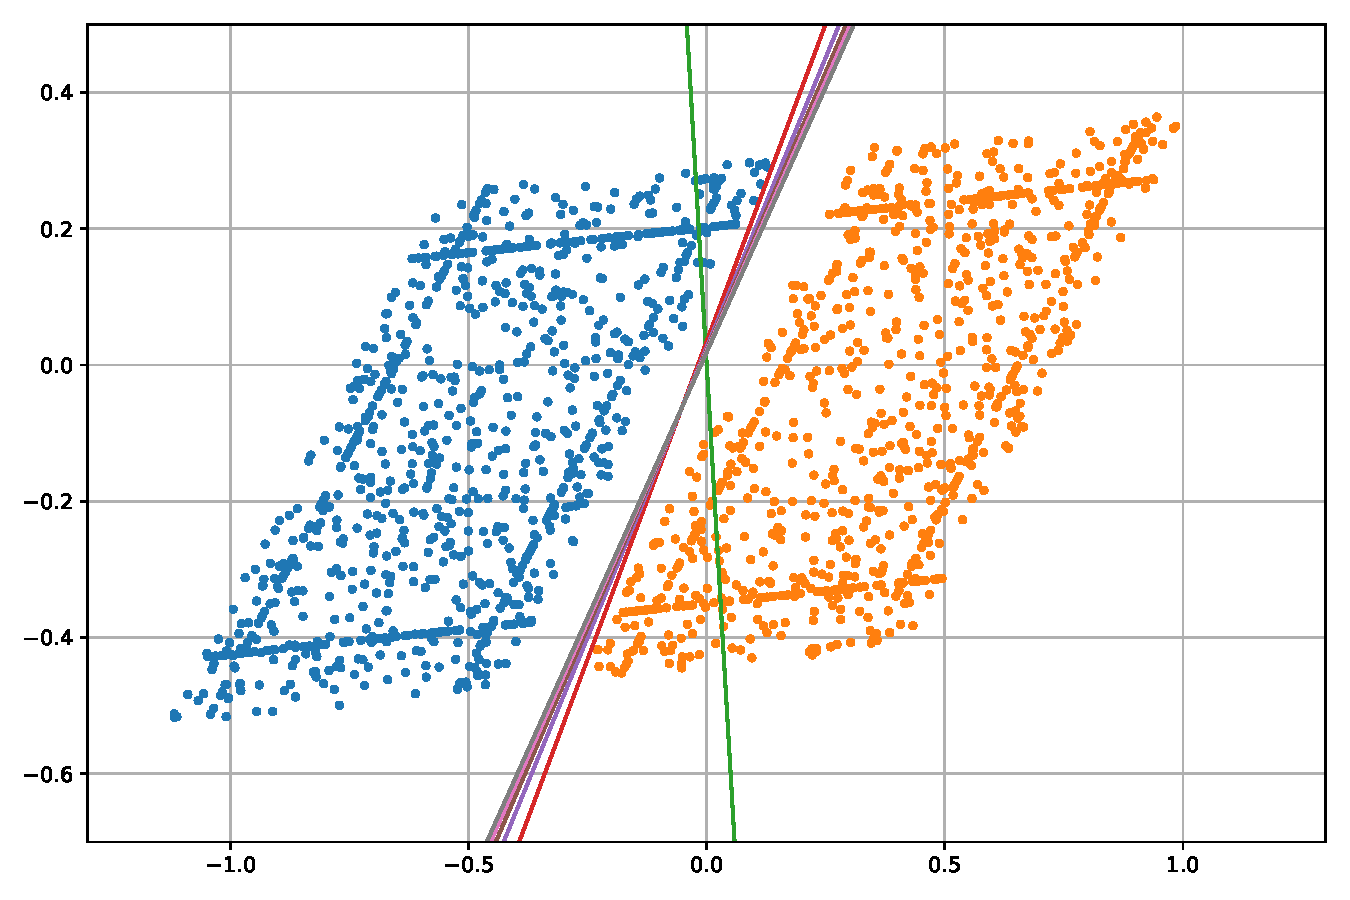
\includegraphics[width=0.5\linewidth]{logistic}
	\caption{Gradient Decent of Logistic Regression}
\end{figure}

Increasing the maximum number of iterates will let the decision boundary converge to the desired boundary, after the loss is 0, the boundary will not change anymore.

Increasing the learning rate will change the step size, a learning rate that is too large may leads to oscillation and one that is too small may leads to slow convergence.

\subsection*{(b) Perceptron} 
\begin{figure}[h]
	\centering
	\subfigure[(i)Perceptron Online Mode]{
		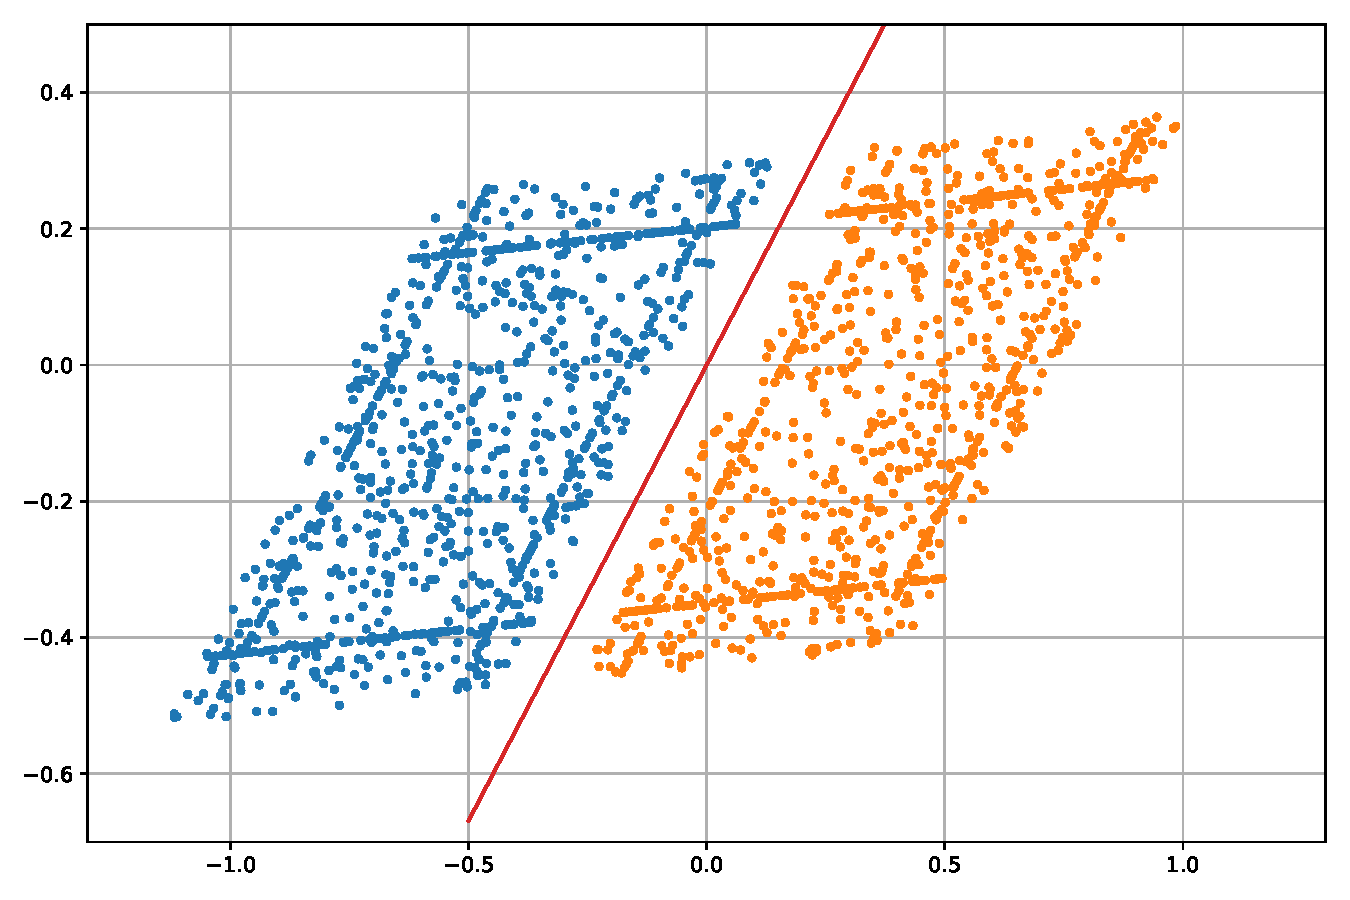
\includegraphics[width=0.47\linewidth]{perceptron_online}
	}
	\subfigure[(ii)Perceptron Batch Mode]{
		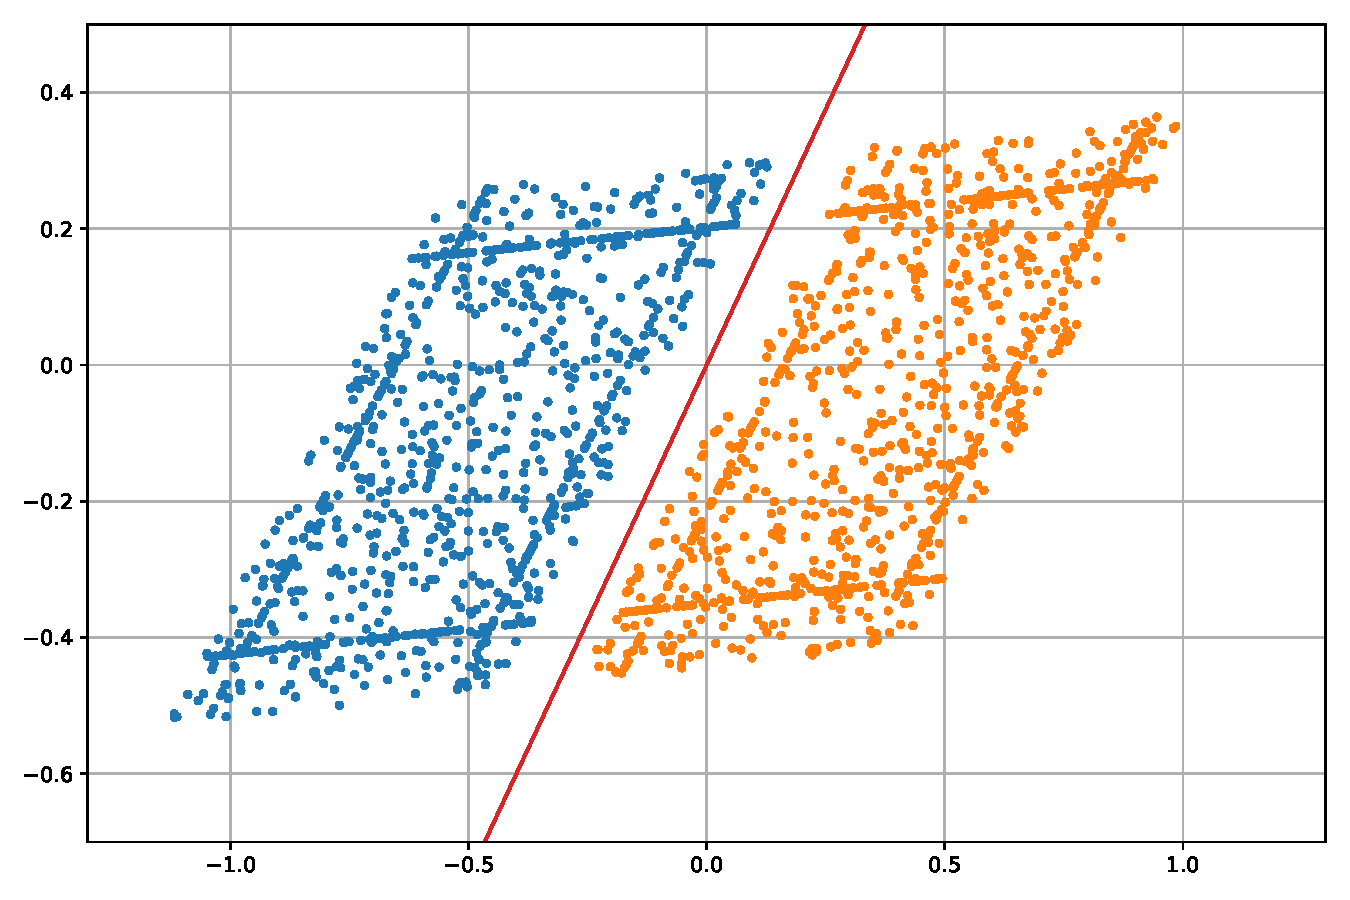
\includegraphics[width=0.47\linewidth]{perceptron_batch}
	}
	\caption{Decision of Perceptron algorithm}
\end{figure}

Batch mode converge faster in term of rounds. However, the cost each round is a lot higher than the online mode.
\pagebreak
\subsection*{(c) SVM}
\begin{figure}[h]
	\centering
	\subfigure[(i)Hard SVM]{
		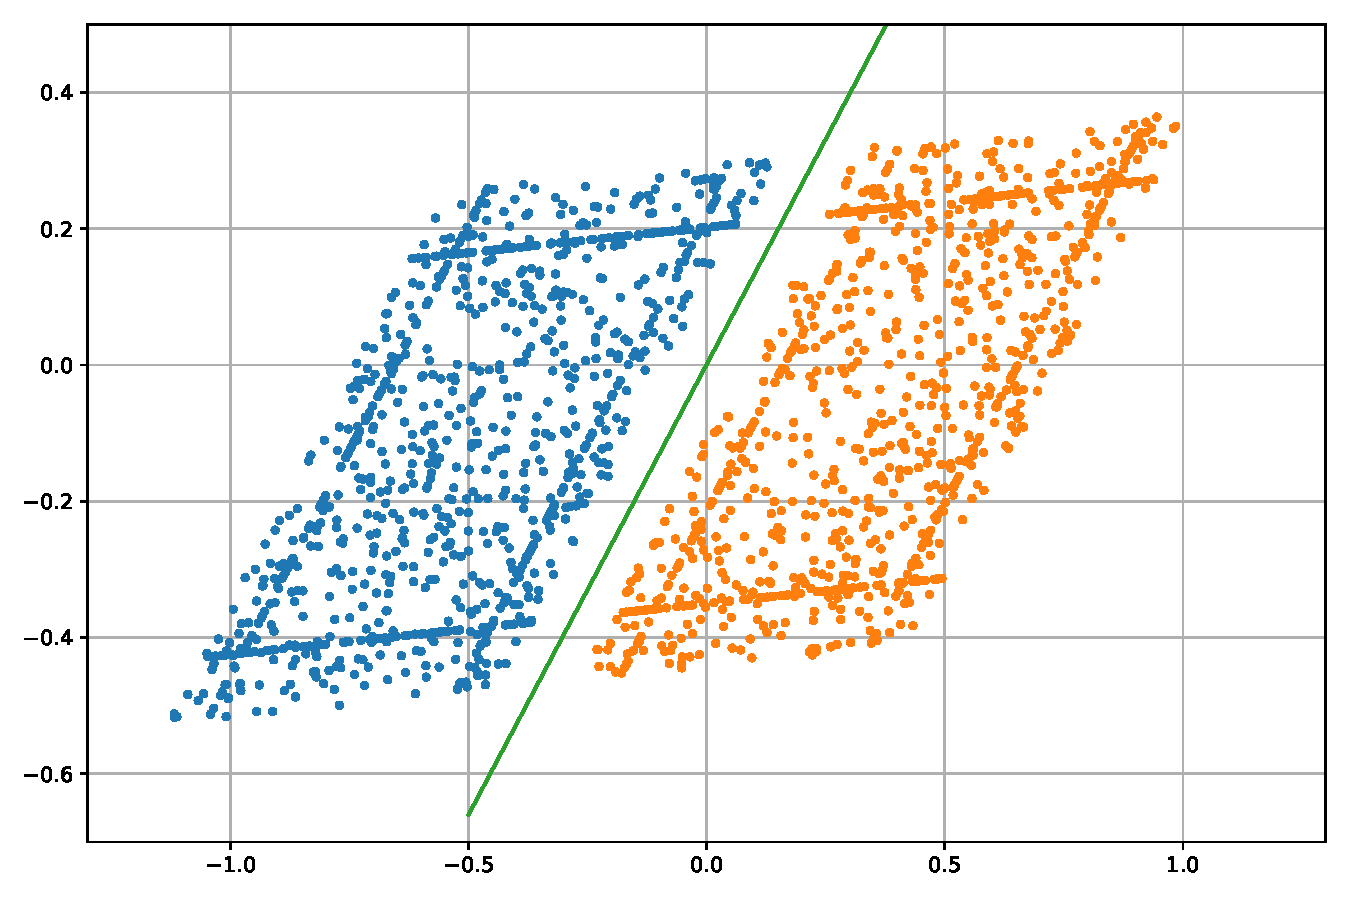
\includegraphics[width=0.47\linewidth]{hardsvm}
	}
	\subfigure[(ii)Soft SVM]{
		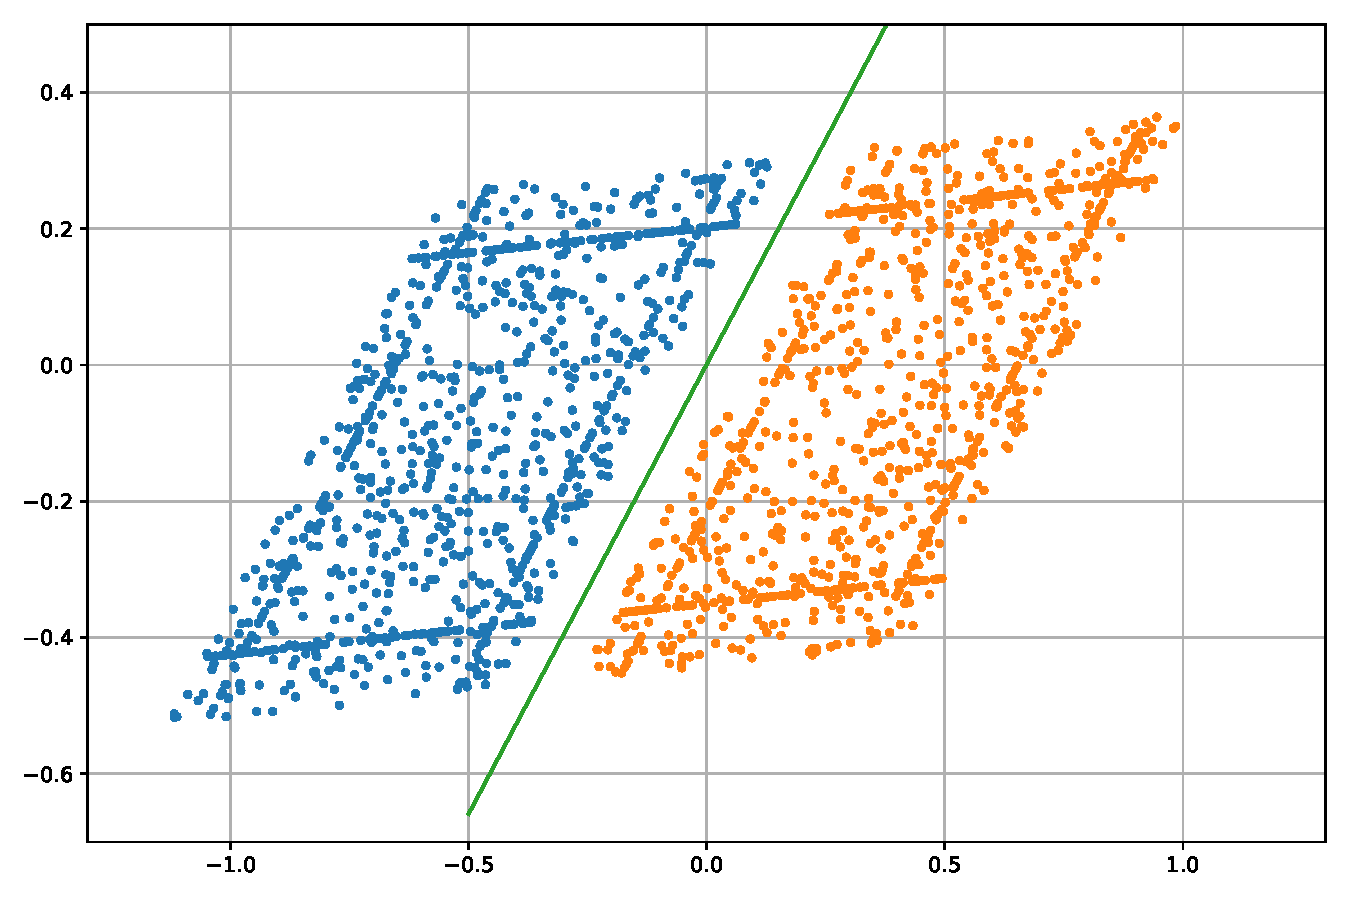
\includegraphics[width=0.47\linewidth]{softsvm}
	}
	\caption{Decision boundary of SVM}
\end{figure}
In this case, the final decision boundary for the soft case is no better than the hard case, since the data is linearly separable.

C is the strength of regularization. Since there is no data point actually goes inside the margin, C is useless in this case.

\subsection*{(d) Comments}

In this case, since the data are linearly separable, the performance of each classifier is pretty much the same. 

In terms of margin, perceptron is not as robust as the other two, in terms of providing a "good" decision boundary and from the graph we can see it has the smallest margin, also it is not a deterministic approach. The other both performs well, while SVM will obviously have larger margin.

However, larger margin does not necessarily means better performance, since over-fitting might be a problem here.   

In all those classifiers, Soft SVM takes the longest to run.
\pagebreak
\section*{Code}

\inputminted[breaklines]{python}{./py/exercise2.py}


\end{document}